\documentclass[declaration,shortabstract,english,inz]{iithesis}
\usepackage[utf8]{inputenc}

%%%%% Tittle page
\polishtitle    {Tworzenie agenta kierującego pojazdem w wirtualnym środowisku TORCS}
\englishtitle   {Developing car driving agent in the TORCS virtual environment }
\polishabstract {\ldots}
\englishabstract{\ldots}
\author         {Kacper Kulczak}
\advisor        {dr Paweł Rychlikowski}
% \date          {}                      %Date
\transcriptnum {279079}
\advisorgen    {dr. Pawła Rychlikowskiego}
%%%%%

%%%%% packages
\usepackage{
    graphicx,
    listings,
    hyperref,
    array,
    longtable,
    wrapfig,
    amsmath,
    algorithmic
    % amssymb,
    % amsthm,
    % amsfonts,
    % tikz 
}
%%%%% Definitions and commands
%
%\theoremstyle{definition} \newtheorem{definition}{Definition}[chapter]
%\theoremstyle{remark} \newtheorem{remark}[definition]{Observation}
%\theoremstyle{plain} \newtheorem{theorem}[definition]{Theorem}
%\theoremstyle{plain} \newtheorem{lemma}[definition]{Lemma}
%\renewcommand \qedsymbol {\ensuremath{\square}}
% ...
%%%%%

\begin{document}

%%%%% BEGINNING

\chapter{Introduction}

Autonomous cars are a very fashionable subject. The idea has a lot of benefits. Most of accidents on roads, occurs due to human mistakes. Programmes don't get tiered or distracted while driving a vehicle. Also they can save a lot of fuel with optimal decisions.
That's why companies around the globe put a lot of effort into making the car software for autonomous driving. It is very interesting task from artificial intelligence perspective. Description of the world is huge. It includes near objects, borders of the street, speed, turning force, engine rotation and much more. The output of such programme is quite simple in compared to the input size. We need only to specify new position of steering wheel and decision if we want to speed up or slow down. During my work I wanted approach the problem by building my own agent capable of drive safely on a racing track.




\section{TORCS Environment}
"The online racing car simulator"(TORCS) is highly portable, multi platform car simulator, with various cars and tracks.  The simulation features a simple damage model, collisions, fuel consumption, tire and wheel properties (springs, dampers, stiffness), aerodynamics and much more \cite{TORCS}.  It is designed to enable programed agents compete against each others. There is very ditalied instruction on developing your  own bot. It has to be written as C++ loadable library and it is attached to main thread during program startup.


\begin{figure}[h]
    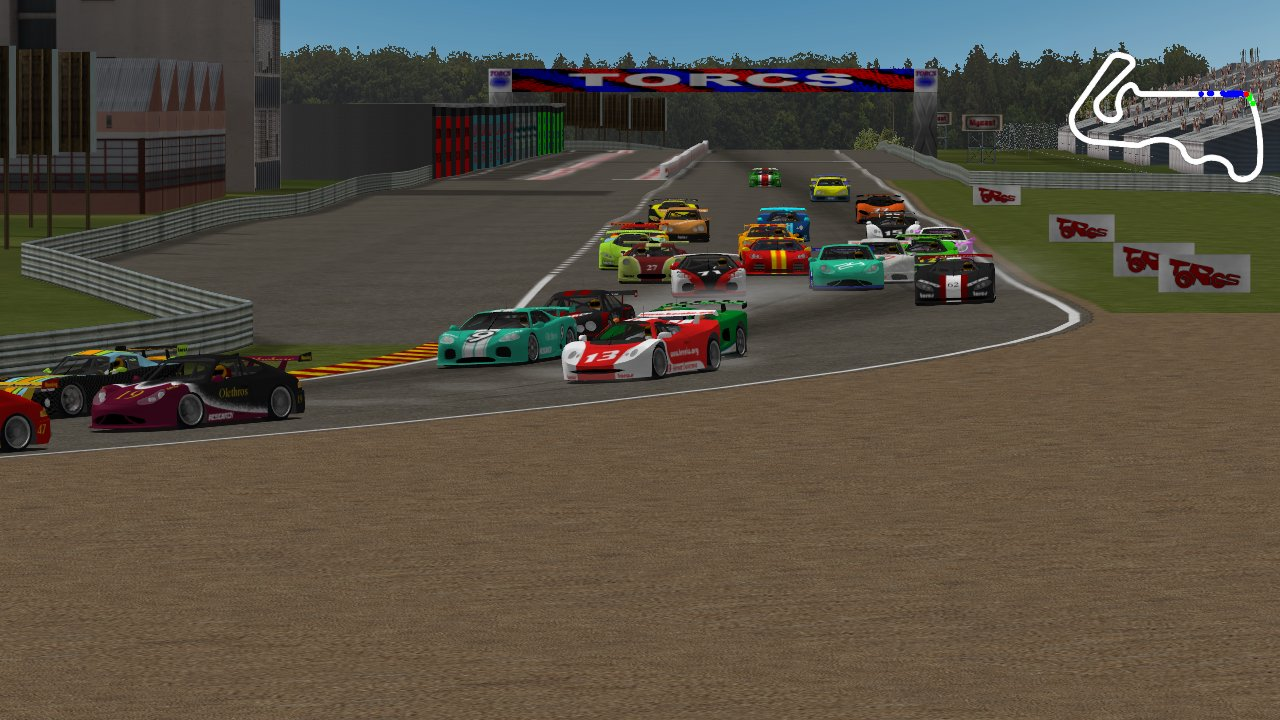
\includegraphics[width=\linewidth]{img/torcs_look.jpeg}
    \caption{Screen shot from TORCS race \cite{TORCS}}
    \label{fig:torcs}
\end{figure}
I have much more experience with programing in high level languages, so clean TORCS environment did not meet all my expectations. 


\section{Simulated Car Racing Championship}

SCRC competition took place between 2007 - 2015 with some breaks. It was organized by the University of Adelaide and the Politecnico de Milano. They used TORCS engine for competition, but organizers provided official patch which changed architecture of the programme. After patching, TORCS became client-server application which allows multiple bots communicate with game engine via UDP connections. 

\begin{wrapfigure}{R}{0.6\textwidth}
    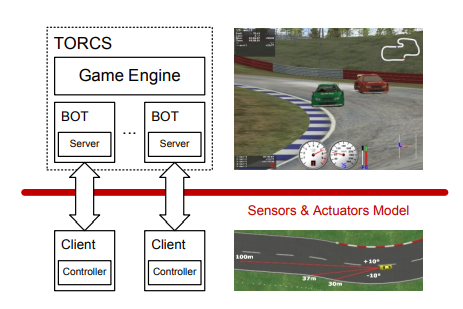
\includegraphics[width=0.55\textwidth]{img/scr_architecture.png}
    \caption{Simulated Car Racing Championship - architecture overview \cite{scrc_manual}}
    \label{fig:scrc_arc}
\end{wrapfigure}

Server sends current sensor inputs (track border, speed, lap time, etc...) and waits for 20ms for the client action (gas, break, steer, etc...). API is details are descrived in table from manual. With that change participants cant choose whatever language they want. That's why I decided to use patched version of TORCS game engine in version 1.3.7

Organizers provided "clients" programmes only in Java and C++. I didn't want to implement communication interface on my own, beacuse it's time consuming  and uninteresting task. After some research,  I found \url{http://xed.ch/p/snakeoil} project, which provides Python Class handling communication with TORCS server. It allowed me to add layer of abstraction and focus directly on driving functionality.

\section{Game sensors and actions parametes}
    
Server provides very accurate description of virtual environment state. All parameters are described in \ref{tab:torcs_sensors} \ref{tab:torcs_actions} table attached to SCRC competition manual \cite{scrc_manual}. 

\begin{center}
    \begin{longtable}{ | p{0.18\textwidth} |p{0.25\textwidth}| p{0.57\textwidth} |}
     \hline
     \textbf{Name} & \textbf{Range (unit)} & \textbf{Description} \\ 
     \hline
     angle & $[-\pi, +\pi]$ (rad) & Angle between the car direction and the direction the track axis. \\  
     \hline
     curLapTime & $[0, +\infty)$ (s) & Time elapsed during current lap. \\
     \hline
     damage & $(0, +\infty)$ (point) & Current damage of the car (the higher is the value the higher is the damage). \\
     \hline
     distFromStart & $[0, +\infty)$ (m) & Distance of the car from the start line along the track line. \\
     \hline
     distRaced & $[0, +\infty)$ (m) & Distance covered by the car from the beginning of the race \\
     \hline
     focus & $[0, 200]$ (m) & Vector of 5 range finder sensors: each sensor returns the distance between the track edge and the car within a range of 200 meters. When noisy option is enabled (see Section 7) sensors are affected by i.i.d. normal noises with a standard deviation equal to the $1\%$ of sensors range. The sensors sample, with a resolution of one degree, a five degree space along a specific direction provided by the client (the direction is defined with the focus command and must be in the range $[-90,+90]$ degrees w.r.t. the car axis). Focus sensors are not always available: they can be used only once per second of simulated time. When the car is outside of the track (i.e., pos is less than $-1$ or greater than $1$), the focus direction is outside the allowed range ($[-90,+90]$ degrees) or the sensors has been already used once in the last second, the returned values are not reliable (typically $-1$ is returned). \\
     \hline
     fuel & $[0, +\infty)$ (l) & Current fuel level. \\
     \hline
     gear & $ \{ -1,0,1, \dots, 6 \} $ & Current gear: -1 is reverse, 0 is neutral and the gear from 1 to 6. \\
     \hline
     lastLapTime & $[0, +\infty)$ (s) & Time to complete the last lap \\
     \hline
     opponents & $[0, 200]$ (m) & Vector of 36 opponent sensors: each sensor covers a span of 10 degrees within a range of 200 meters and returns the distance of the closest opponent in the covered area. When noisy option is enabled, sensors are affected by i.i.d. normal noises with a standard deviation equal to the $2\%$ of sensors range. The 36 sensors cover all the space around the car, spanning clockwise from $-180$ degrees up to $+180$ degrees with respect to the car axis. \\
     \hline
     racePos & $\{1,2,\dots,N\}$ & Position in the race with respect to other cars. \\
     \hline
     rpm & $[0, +\infty)$ (rpm) & Number of rotation per minute of the car engine \\
     \hline
     speedX & $ ( -\infty, +\infty ) $ (km/h) & Speed of the car along the longitudinal axis of the car. \\
     \hline
     speedY & $ ( -\infty, +\infty ) $ (km/h) & Speed of the car along the transverse axis of the car. \\
     \hline
     speedZ & $ ( -\infty, +\infty ) $ (km/h) & Speed of the car along the Z axis of the car \\
     \hline        
     track &  $[0, 200]$ (m) & Vector of 19 range finder sensors: each sensors returns the distance between the track edge and the car within a range of 200 meters. When noisy option is enabled, sensors are affected by i.i.d. normal noises with a standard deviation equal to the $10\%$ of sensors range. By default, the sensors sample the space in front of the car every 10 degrees, spanning clockwise from $-90$ degrees up to $+90$ degrees with respect to the car axis. However, the configuration of the range finder sensors (i.e., the angle w.r.t. to the car axis) can be set by the client once during initialization, i.e., before the beginning of each race. When the car is outside of the track (i.e., pos is less than $-1$ or greater than $1$), the returned values are not reliable (typically $-1$ is returned). \\
     \hline
     trackPos & $( -\infty, +\infty )$ & Distance between the car and the track axis. The value is normalized w.r.t to the track width: it is $0$ when car is on the axis, $-1$ when the car is on the right edge of the track and $+1$ when it is on the left edge of the car. Values greater than $1$ or smaller than $-1$ mean that the car is outside of the track. \\
     \hline
     wheelSpinVel & $[0, +\infty)$ (rad/s) & Vector of 4 sensors representing the rotation speed of wheels. \\
     \hline
     z & $( -\infty, +\infty ) $ (km/h) & Distance of the car mass center from the surface of the track
     along the Z axis \\
     \hline
     \caption{\label{tab:torcs_sensors}: Description of the available sensors.}
    \end{longtable}

\end{center}

\begin{center}
    \begin{longtable}{ | p{0.18\textwidth} |p{0.25\textwidth}| p{0.57\textwidth} |}
    \hline
    \textbf{Name} & \textbf{Range (unit)} & \textbf{Description}  \\ 
    \hline
    accel & $[0,1]$ & Virtual gas pedal (0 means no gas, 1 full gas). \\ 
     \hline
     brake &  $[0,1]$ & Virtual brake pedal (0 means no brake, 1 full brake). \\ 
     \hline
     clutch &  $[0,1]$ & Virtual clutch pedal (0 means no clutch, 1 full clutch). \\ 
     \hline
     gear & $\{-1,0,1,\dots ,6\}$ & Gear value. \\ 
     \hline
     steer &  $[-1,1]$ & Steering value: $-1$ and $+1$ means respectively full right and
     left, that corresponds to an angle of $0.366519$ rad. \\ 
     \hline
     focus &  $[-90,90]$ & Focus direction (see the focus sensors) in degrees. \\ 
     \hline
     endRace &  $\{0,1\}$ & This is meta-control command: 0 do nothing, 1 ask competition
     server to restart the race. \\ 
     \hline
     \caption{\label{tab:torcs_actions}Description of the available  action parameters.}
    \end{longtable}
\end{center}

\chapter{Standard programing approach}

\section{Line follower}

The first approach to the problem was developing simple bot which follows the track axis. Every time, absolute value of trackPos sensor (normalized position of the car on the track between $[-1, +1]$) is bigger than given small threshold, agent turns towards axis of the track with turning force set to 35\%. To avoid zigzag driving, very small course corrections are applied, whenever $abs(trackPos) < 0.2$. Speed is limited to 80 km/h. These configuration allows bot to safely drive on every track. 

I am aware that limiting turing force, has huge negative impact on bot performance. However increasing that value leads to dangerous behaviors. I was surprised how easy it is to slip. During development line follower I haven't found any solution for getting out of the slip. For now limiting that value was necessary.

\section{Speed limit signs}

In real world, government for safety reasons, places speed limit sign on dangerous sectors of roads. Signs are placed before sharp turns, steep slopes, bridges, viaducts, and more. Drivers adjust the speed to specific environment conditions. Inspired by this observation, I tried to improve previous agent iteration. 

I've split the track on 8 sections, using distFromStart sensor (distance of the car from the start line along the track line). Every part would have different speed limit set for specific track. The goal is to finish the lap as fast as we can while not falling out of the track. So we need to minimize function $f$, where $l_i$ - speed limit for section $i$ in km/h.

$$ f(l_1, l_2, \dots, l_n ) =  \begin{cases}
    \infty &\quad , \text{when the car fell off the track}\\
    \text{lap\_time}  &\quad , \text{otherwise} \\
  \end{cases}
 $$

I was trying to implement genetic algorithm for finding optimal limits for given track, but it appears that game engine, even with turned graphics off, isn't as fast as I anticipated. It takes almost 20 seconds, to complete one lap. Simple genetic algorithm would need long hours to find approximately good solution. I've used two following observations while developing my algorithm.

\begin{itemize}
    \item  $l_i \in [40, 300]$:  Smaller values can lead to disqualification from race.
    \item  true speed of car on sction $i$, depends on $l_i$ and true speed at the end of section $i-1$
    \item
    $l_i$ is correct, when $l_{i+1} = 40$ and car didn't fell out from track
    \item  $g_j(x) = f(l_1,l_2, \dots,l_{j-1}, x, l_{j+1}, \dots, l_n)$ is decreasing while car stays on the track
    
\end{itemize}


I've implemented algorithm based on divide and conquer idea. It finds maximal x, where $g(x) \neq \infty$. We run that procedure on every argument:

\begin{algorithmic}
    \STATE $l_i\gets 40$
    \FOR{$i\gets 1,\dots, n$}
        \STATE $l_i = devide\_and\_conquer(func=g_i, min=40, max=300)$
    \ENDFOR
\end{algorithmic}

For every section it uses around 12 game engine runs. So whole algorithm ends execution after around half an hour.

\section{Results and observations}

In following table I've presented line-follower performance on specific tracks from TORCS environment. While speed limits are significant improvement, they still do not deal with major flaw of the concept. Our bot is extremely reactive. Human driver see a turn from distance and prepares for it (reduces speed, drifts towards opposite side of the road). On the other hand my bot turns the steering wheel only when it drifts away from the middle of the track (this happens after entering the turn). It is basically to late for a perfect turning maneuver. We need a model, which predicts and reacts to the  future events. That's why I resign from extending current concept.


\begin{table}[h]
    \centering
    \begin{tabular}{ |c|c|c|}
          \hline
          track name & line-follower [s] & with speed limits [s] \\
          \hline
          forza & $265.51$ & $146.31$  \\
          \hline
          cg\_track\_2 & $148.84$ &  $84.68$\\
          \hline
          cg\_track\_3 & $133.74$ & $91.86$ \\
          \hline
        \end{tabular}
        \caption{Line follower performance for specific TORCS tracks}
        \label{tab:line_follower}

\end{table}

\chapter{Machine Learning Approach}

\section{Collecting the data}

Machine learning is well known 

Unfortunately TORCS environment does not have an option to log sensors data and driver actions. It is planned to add this functionality in the future development. That's why I developed software which mimics TORCS car controls and saves data from all sensors and driver actions to json file. From game perspective it is normal agent, but it reacts only on user keyboard inputs (accelerate, break, left, right).  With that infrastructure I was able to record some well-driven race laps on various tracks.  

\section{Single Classifier}

During 10 recording laps on \textit{cg\_track\_2} I've collected around 30000 data frames. The state passed to classifier is made up of following sensors:

\paragraph{State parameters}
\begin{itemize}
    \item \textbf{speeds} (3 speed sensors in axises x,y,z )
    \item \textbf{angle}, \textbf{trackPos} (same as in line-follower) 
    \item \textbf{track}  (19 sensors in front of the car measuring distances to edge of track) 
    \item \textbf{distFromStart} (distance of the car from the start line along the track line
\end{itemize}

All values are normalized between $[-1,1]$ and combined in a single vector. For actions I've created a list of unique actions present in data set and labeled them. For track \textit{cg\_track\_2} It reduced set of actions to around 200. 

\paragraph{Action parameters}
\begin{itemize}
    \item \textbf{accel} $\in \{0,1\}$
    \item \textbf{brake} $\in \{0,1\}$ 
    \item \textbf{steer} $\in [-1,1]$
\end{itemize}

Classifier for state vector, should answer with label of which action are we supposed to execute. First and actually only successful approach was  simple decision tree classifier from scikit-learn library (implementation of CART algorithm).  Results are shown in table \ref{tab:single_clp_tree}.


\begin{table}[h]
    \centering
    \begin{tabular}{ |c|c|c|}
          \hline
          track name & line-follower with limts [s] & single decision tree classifier [s] \\
          \hline
          cg\_track\_2 & $84.68$ & $61.18$ \\
          \hline
        \end{tabular}
        \caption{Single Classifier: decision tree performance}
        \label{tab:single_clp_tree}

\end{table}

Performance was improved by 20\% even with poor model accuracy. Classifier accuracy on test data set is equal 61\%. Other models such as (Neural Network, Support Vector Machine, Random Forest) resulted in similar bad accuracy for test data set and all of them were getting out from the race track.   

It is worth noticing, that using \textbf{distFromStart} parameter isn't very practical for generalized driving agent. My models weren't learning how to drive a vehicle. The were rather memorizing right actions for specific sector of the track. We need model which can be applied also for unseen tracks. However without that parameter, all my models were crashing on the track.

\section{Two models}

Major flaw for previous classifier was tha amount of possible answers. To reduce number of classes we need to use two seperate models: 

\begin{itemize}
    \item \textbf{Steer Regressor} - responsible for determining the turn rate (floating number between [-1,1]).
    \item \textbf{Acceleration Classifier} - determining
\end{itemize}


\chapter{Adidtonal Problems}

\begin{itemize}
    \item \textbf{Transmission} Choosen architecture didn't allowed me to use automatic transmission included with the torcs game. I had to build my own basic automatic transmission system, which is far from perfect. I haven't change it during development of different agents, so all results are comparable. 
\end{itemize}


%%%% BIBLIOGRAPHY

\begin{thebibliography}{1}
\bibitem{TORCS} B. Wymann, E. Espié, C. Guionneau, C. Dimitrakakis, R. Coulom, A. Sumner. TORCS: The Open Racing Car Simulator, v1.3.6, 2014.
\bibitem{scrc_manual} Daniele Loiacono, Luigi Cardamone, Pier Luca Lanzi, “Simulated Car
Racing Championship: Competition Software Manual”, Technical Report 2011.06, Dipartimento
di Elettronica e Informazione, Politecnico di Milano, Italy, 2011.
\end{thebibliography}






\end{document}
